\documentclass[conference]{IEEEtran}

\usepackage[utf8]{inputenc}
\usepackage[T1]{fontenc}
\usepackage{cite}
\usepackage{graphicx}
\usepackage{booktabs}
\usepackage{amsmath}
\usepackage{subcaption}
\usepackage{url}
\usepackage{hyperref}
\usepackage{float}

\title{HypRID - Hyperspectral Radar Imaging Dataset}

\author{
    \IEEEauthorblockN{Steven Chen, Yung-Hsin Tsai}
    \IEEEauthorblockA{
        Department of Electrical and Computer Engineering \\
        Rice University \\
        Houston, TX, USA
    }
}

\begin{document}

\maketitle

\begin{abstract}
HypRID is a multimodal sensing project aimed at supporting future radar-enhanced 3D perception. Since the midterm stage, the project has shifted from immediate dataset collection toward evaluating existing depth-estimation, radar-depth, and radar-camera fusion models to better guide future model and dataset design. The sensing system was also updated with a TI AWR2243 76--81 GHz FMCW radar board, which has been mounted and hardware-tested as an additional radar modality. Qualitative model evaluations showed that Depth Anything V2 produced the most promising RGB-based depth results among the tested models, while stereo models such as RAFT-Stereo and HITNet were poorly matched to the current D415 IR stereo setup. RadarHD was also evaluated on ColoRadar data, but produced incomplete outputs due to dataset and preprocessing mismatch. These findings suggest a future model direction that fuses RGB image guidance with 2D and 3D radar point clouds to generate high-resolution depth maps.
\end{abstract}

\section{Introduction}

Reliable 3D scene understanding is an important requirement for autonomous systems, robotics, and intelligent sensing platforms operating in real-world environments. Many existing perception systems rely heavily on optical sensors, such as RGB cameras, RGB-D sensors, or stereo cameras. Although these sensors can provide dense visual information, their performance can degrade under difficult lighting, reflective or transparent surfaces, thin structures, occlusion, and other challenging sensing conditions. Radar-based sensing can provide complementary information that is less dependent on visible-light conditions, making it a valuable modality for robust 3D perception \cite{guan2020through}.

To explore this direction, we propose \textit{HypRID - Hyperspectral Radar Imaging Dataset}, a multimodal sensing project focused on radar-enhanced depth perception. In this project, \textit{hyperspectral} refers to the combination of multiple sensing modalities rather than traditional optical hyperspectral imaging. The long-term goal of HypRID is to combine RGB imaging, optical depth sensing, 2D radar, 3D radar, and LiDAR ground truth to support future model development for high-resolution depth-map generation and downstream 3D perception tasks. The midterm stage of the project established the initial hardware platform and demonstrated preliminary calibration between the 300--330 GHz radar and Intel RealSense D415. Since then, the project direction has shifted from immediate dataset collection toward model review and evaluation, so that future data collection can be guided by a clearer downstream modeling objective.

The current system includes a 300--330 GHz radar, an Intel RealSense D415 RGB-D sensor, and a newly mounted TI AWR2243 76--81 GHz FMCW radar board. The TI board adds a lower-frequency radar modality to the system, allowing future work to compare and fuse information from different radar frequency bands. The Ouster OS0-128 LiDAR remains part of the planned sensing suite and will serve as a future geometric ground-truth reference. Although full dataset collection has not yet started, the updated system provides a stronger foundation for future multimodal data capture.

The main progress after the midterm report was a literature-review and qualitative model-evaluation stage. RGB-based depth estimation models, including Depth Anything V2 and MiDaS, were evaluated to understand their robustness in difficult regions such as transparent surfaces, reflective areas, and thin structures \cite{yang2024depthanythingv2,ranftl2022towards}. Stereo models, including RAFT-Stereo and HITNet, were tested using the current D415 image pairs to determine whether they fit the existing sensing setup \cite{lipson2021raft,tankovich2021hitnet}. RadarHD was also evaluated using adapted ColoRadar data to study the transferability of radar depth-map models across datasets \cite{prabhakara2023high,kramer2022coloradar}. Finally, MetaMoran was reviewed as a relevant radar-camera fusion method because it uses RGB segmentation and depth estimation to guide radar-based depth imaging \cite{prabhakara2022metamoran}.

These studies suggest that a promising future direction for HypRID is to fuse RGB image information with both 2D and 3D radar point clouds to generate a high-resolution depth map. In this direction, RGB-based segmentation and depth estimation can provide structural and semantic guidance, while radar point clouds can provide complementary geometric information. Compared with prior radar-camera fusion approaches based on 2D radar, the HypRID system may benefit from the elevation information and finer spatial detail provided by 3D radar sensing. This final report summarizes the updated sensing system, the post-midterm model evaluation process, the qualitative results, and the resulting design direction for future HypRID development.

\section{Methods}

\subsection{Updated System Setup}

The current HypRID system builds on the midterm prototype by adding a TI AWR2243 76--81 GHz FMCW radar board to the sensing platform. The updated system now includes the 300--330 GHz radar, the Intel RealSense D415 RGB-D sensor, and the TI radar board. The TI board has been physically mounted and hardware-tested, and the system is capable of collecting raw radar data that can later be post-processed into range profiles, point clouds, and heatmaps. The Ouster OS0-128 LiDAR remains part of the planned system and is intended to serve as a future ground-truth geometric reference.

Table~\ref{tab:sensors} summarizes the current sensing components and their roles in the final project stage. Figure~\ref{fig:system} shows the updated sensing platform.

\begin{table}[t]
\centering
\caption{Current sensing components in the HypRID system.}
\label{tab:sensors}
\begin{tabular}{p{0.27\columnwidth}p{0.28\columnwidth}p{0.34\columnwidth}}
\toprule
Sensor & Type / Frequency & Current Status / Role \\
\midrule
300--330 GHz radar & Sub-THz radar & Mounted, available for scans \\
TI AWR2243 & 76--81 GHz FMCW radar & Mounted, hardware-tested \\
Intel RealSense D415 & RGB-D sensor & Mounted, RGB/depth collection \\
Ouster OS0-128 & 3D LiDAR & Future ground-truth sensor \\
\bottomrule
\end{tabular}
\end{table}

\begin{figure}[t]
    \centering
    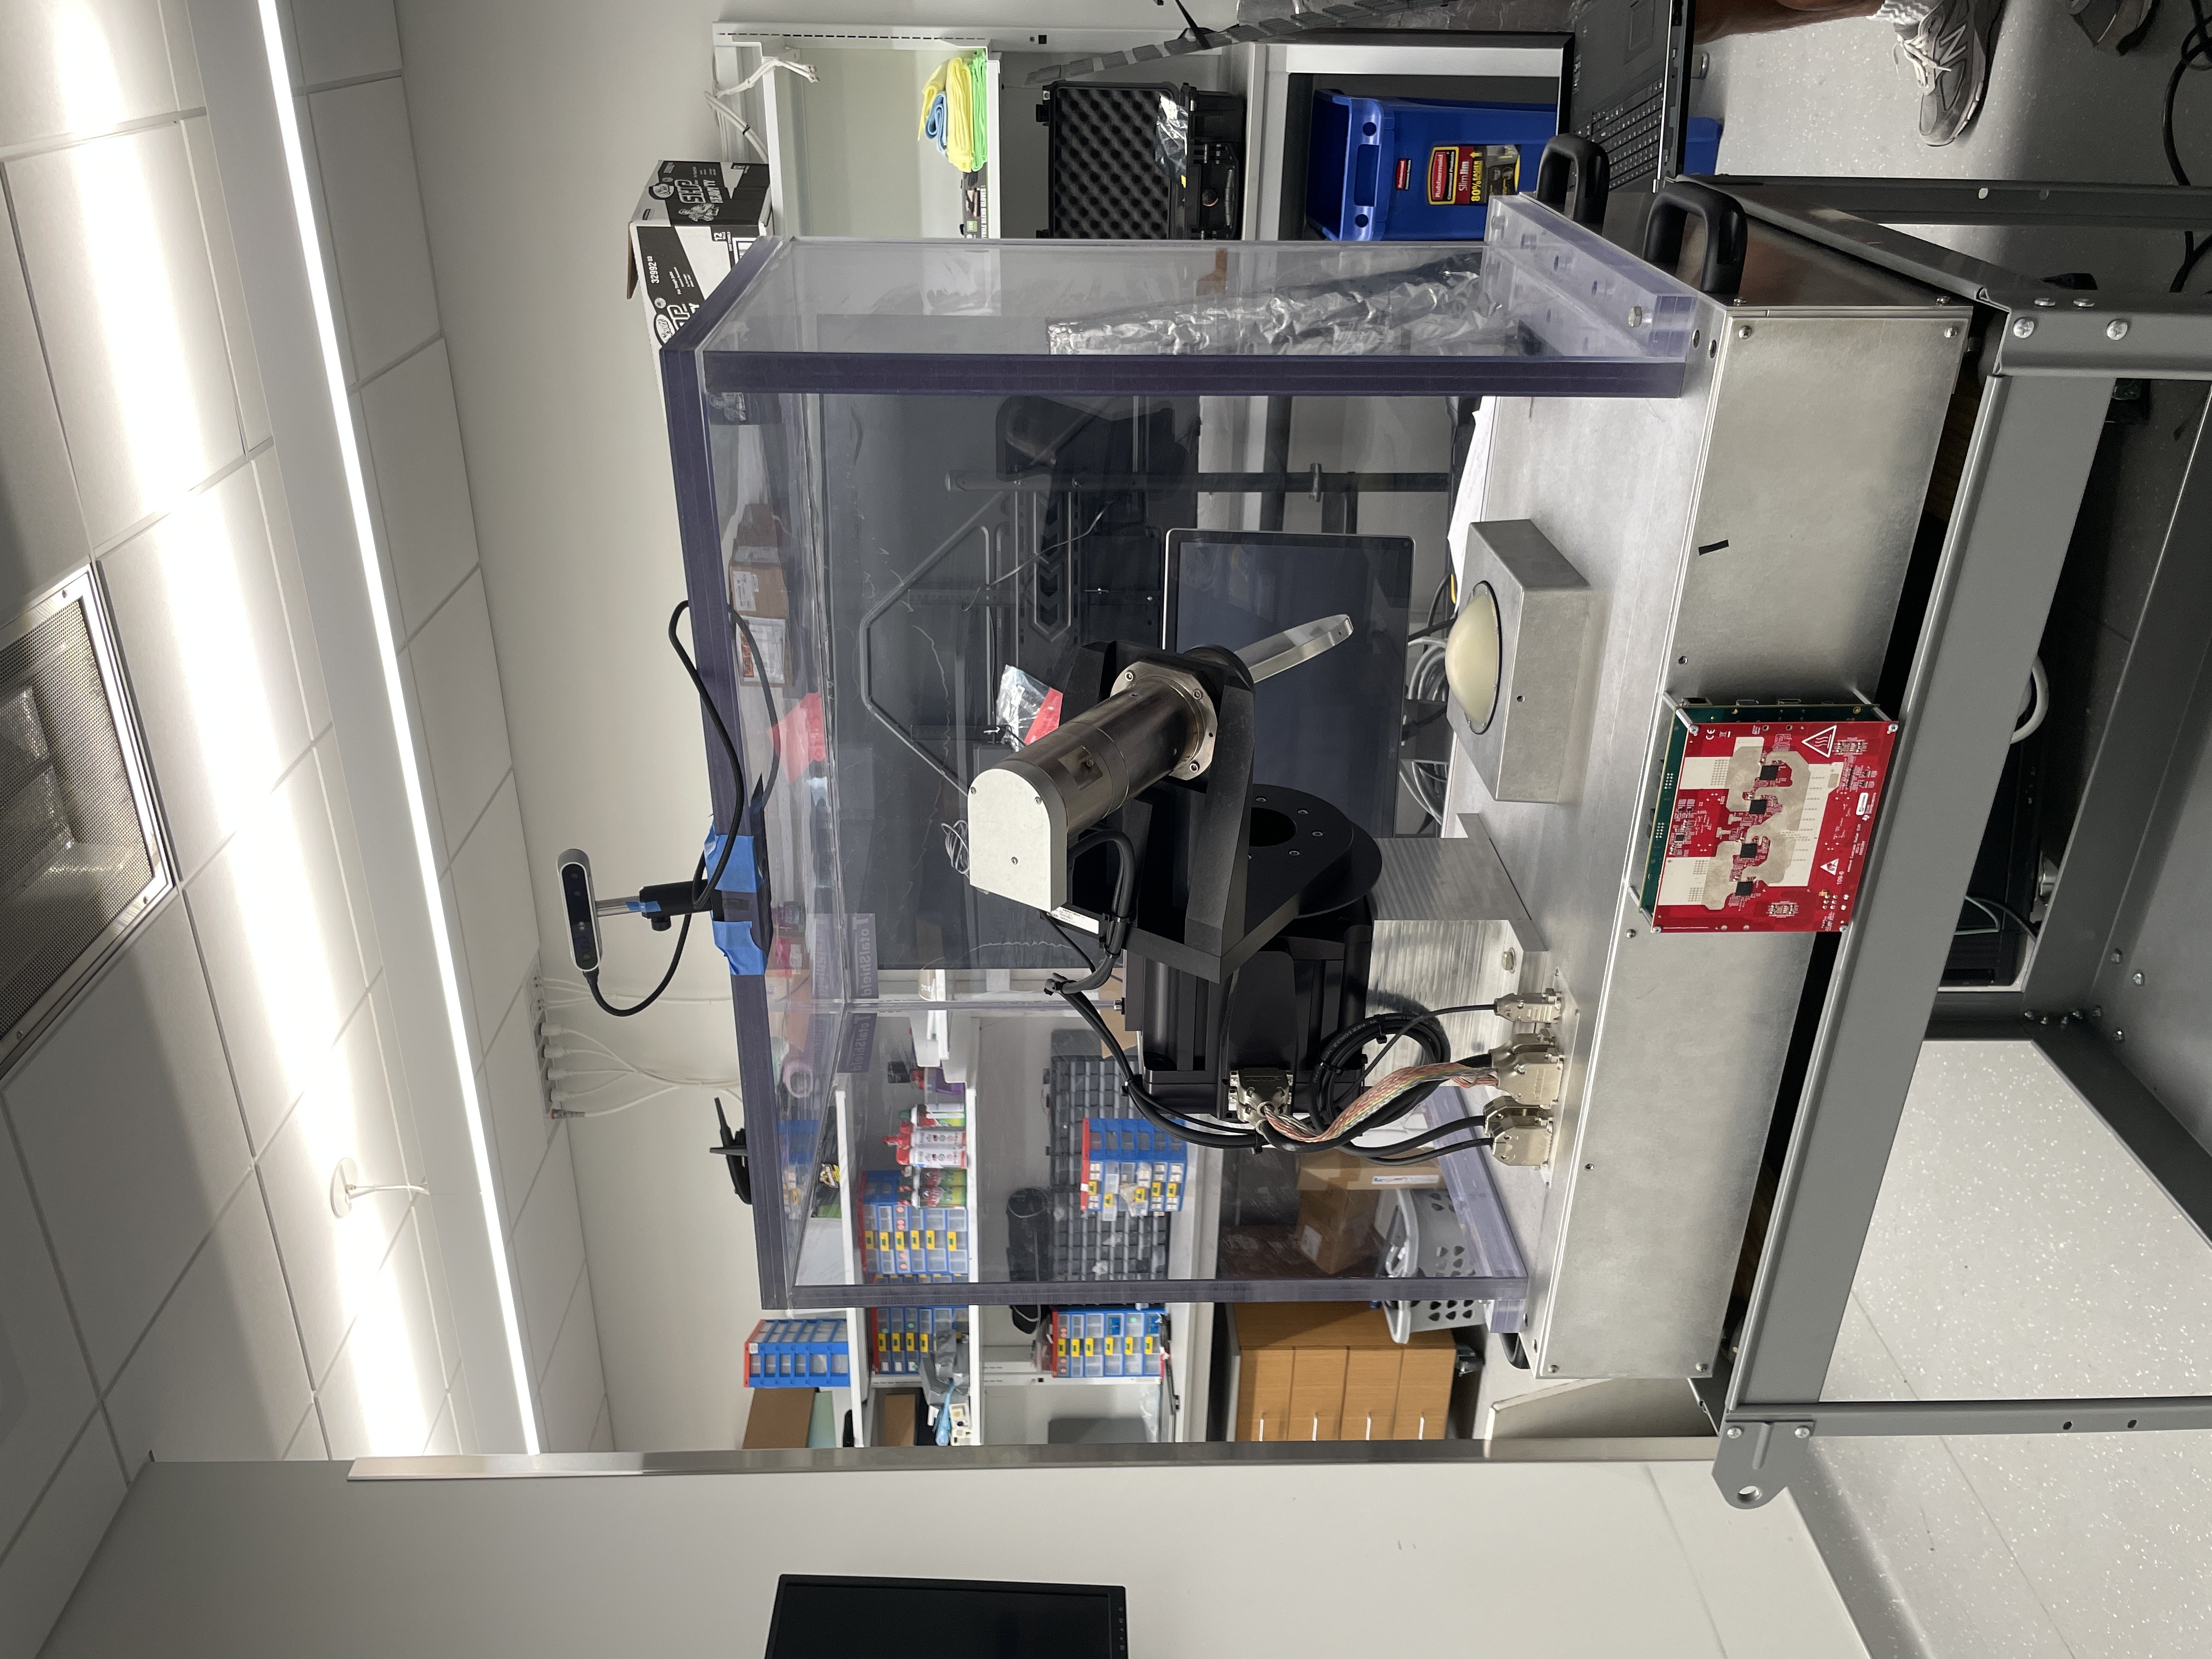
\includegraphics[width=0.75\columnwidth,angle=-90]{figures/updated_system_setup.jpg}
    \caption{Updated HypRID sensing platform. The system now includes the 300--330 GHz radar, the Intel RealSense D415, and the mounted TI AWR2243 76--81 GHz FMCW radar board.}
    \label{fig:system}
\end{figure}

\subsection{Model Review and Evaluation Strategy}

After the midterm stage, the project focus shifted from immediate dataset collection toward reviewing and evaluating existing models to guide future system and dataset design. This shift was necessary because the dataset should be collected with a clearer downstream objective rather than being designed only around available sensors. The reviewed work was grouped into three categories: RGB-based depth estimation, radar depth-map generation, and radar-camera sensor fusion.

The evaluation was qualitative rather than quantitative. No ground-truth depth maps were available for the tested scenes, and the purpose of the evaluation was not to produce a final benchmark. Instead, the goal was to determine which model directions appear most compatible with HypRID and which limitations should influence future model design. The qualitative evaluation focused on whether the model outputs preserved object structure, thin geometry, transparent or reflective regions, and overall scene layout.

\subsection{RGB Depth Estimation Evaluation}

RGB-based depth estimation was evaluated using monocular and stereo models. The monocular models included Depth Anything V2 and MiDaS \cite{yang2024depthanythingv2,ranftl2022towards}. The stereo models included RAFT-Stereo and HITNet \cite{lipson2021raft,tankovich2021hitnet}. Two representative scenes were tested: an indoor scene containing a metal sphere and an outdoor scene containing tree branches with windows in the background. These scenes were selected because they contain structures that are relevant to the HypRID sensing problem, including reflective objects, thin structures, and transparent or visually complex regions.

For the monocular models, each RGB input image was processed to produce a relative depth map. The outputs were visually compared with the original scene to evaluate whether object boundaries, relative depth ordering, and fine structures were preserved. For stereo models, the current available stereo input came from the Intel RealSense D415 IR image pair rather than from a custom RGB stereo camera. This created a domain mismatch because RAFT-Stereo and HITNet are designed and trained primarily for RGB stereo imagery. The purpose of testing these models was therefore to determine whether existing stereo models could be directly applied to the current HypRID setup.

\subsection{Radar Depth Map Evaluation}

RadarHD was evaluated as a representative radar depth-map or radar point-cloud enhancement model \cite{prabhakara2023high}. Since the original RadarHD data collection setup was not available, ColoRadar was used as an available external radar dataset for testing \cite{kramer2022coloradar}. ColoRadar data were extracted and post-processed to fit the input format expected by RadarHD. After this adaptation, the model was able to run successfully.

However, the resulting output was incomplete and worse than expected. This evaluation was useful because it showed that radar depth-map models may not transfer directly across radar datasets without carefully matching the original data format, preprocessing pipeline, and training distribution. The RadarHD experiment therefore helped identify dataset compatibility and model generalization as important considerations for future HypRID model development.

\subsection{Sensor Fusion Review}

MetaMoran was reviewed as the main sensor-fusion reference because it combines mmWave radar and RGB camera information for long-range depth imaging \cite{prabhakara2022metamoran}. The method uses image segmentation and monocular depth estimation to guide radar processing, which makes it closely related to the future direction of HypRID. However, MetaMoran relies on a 2D radar setup, so its depth imaging is limited in the elevation dimension.

This limitation is directly relevant to HypRID. The HypRID system is designed around both lower-frequency 2D radar and higher-resolution 3D radar sensing. While the working range of the 300--330 GHz radar may be shorter than long-range outdoor mmWave systems, its higher angular and range resolution may provide more useful geometric detail for static-scene reconstruction. The sensor fusion review therefore suggests a future model direction in which RGB-based segmentation and depth estimation provide visual guidance, while 2D and 3D radar point clouds provide complementary geometric information.

\section{Results}

\subsection{Updated System Integration}

The updated system now includes the TI AWR2243 radar board as a new sensing component. Compared with the midterm stage, this is an important hardware update because the system now contains both the 300--330 GHz radar and a lower-frequency 76--81 GHz FMCW radar modality. The TI board has been mounted and hardware-tested successfully, although it has not yet been used for full dataset collection. This update supports the long-term goal of comparing and fusing radar information from different frequency bands.

\subsection{RGB Depth Estimation Results}

Among the tested RGB-based depth estimation models, Depth Anything V2 produced the most visually promising results. As shown in Fig.~\ref{fig:depthanything}, the model generated relative depth maps that preserved major scene structures in both the indoor and outdoor test scenes. In the indoor scene, the metal sphere remained visible in the predicted depth map. In the outdoor scene, the model preserved thin tree branch structures and produced a coherent representation around the window regions. These are meaningful observations because reflective objects, transparent regions, and thin structures are areas where traditional RGB-D sensing can struggle.

MiDaS was tested on the same two scenes, but its outputs were less structurally consistent and did not reproduce the tree or sphere as clearly. Because the MiDaS results did not provide additional useful visual evidence, they are discussed as a baseline but not shown as a main figure. Overall, the Depth Anything V2 results suggest that monocular RGB-based depth estimation may provide useful structural guidance for future HypRID fusion models.

\begin{figure}[H]
    \centering

    \begin{subfigure}{0.95\columnwidth}
        \centering
        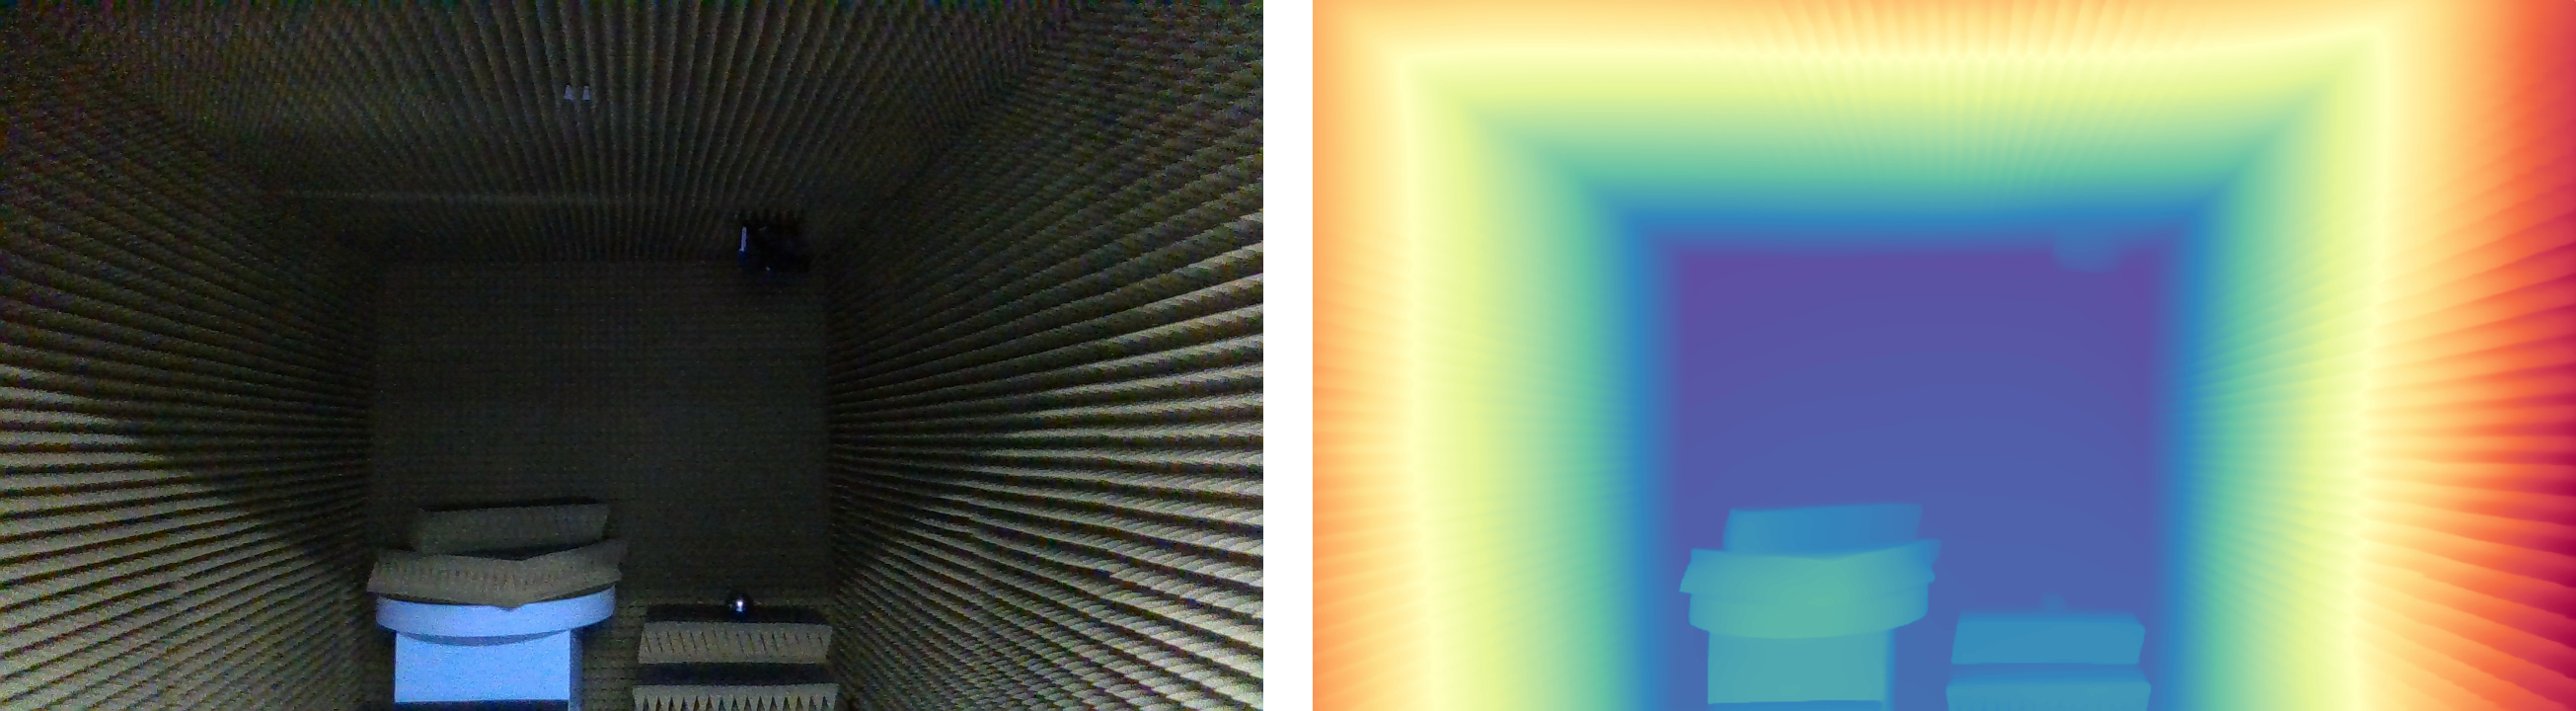
\includegraphics[width=\linewidth]{figures/depthanything_large.png}
        \caption{Indoor scene}
        \label{fig:da_indoor}
    \end{subfigure}

    \vspace{0.4em}

    \begin{subfigure}{0.95\columnwidth}
        \centering
        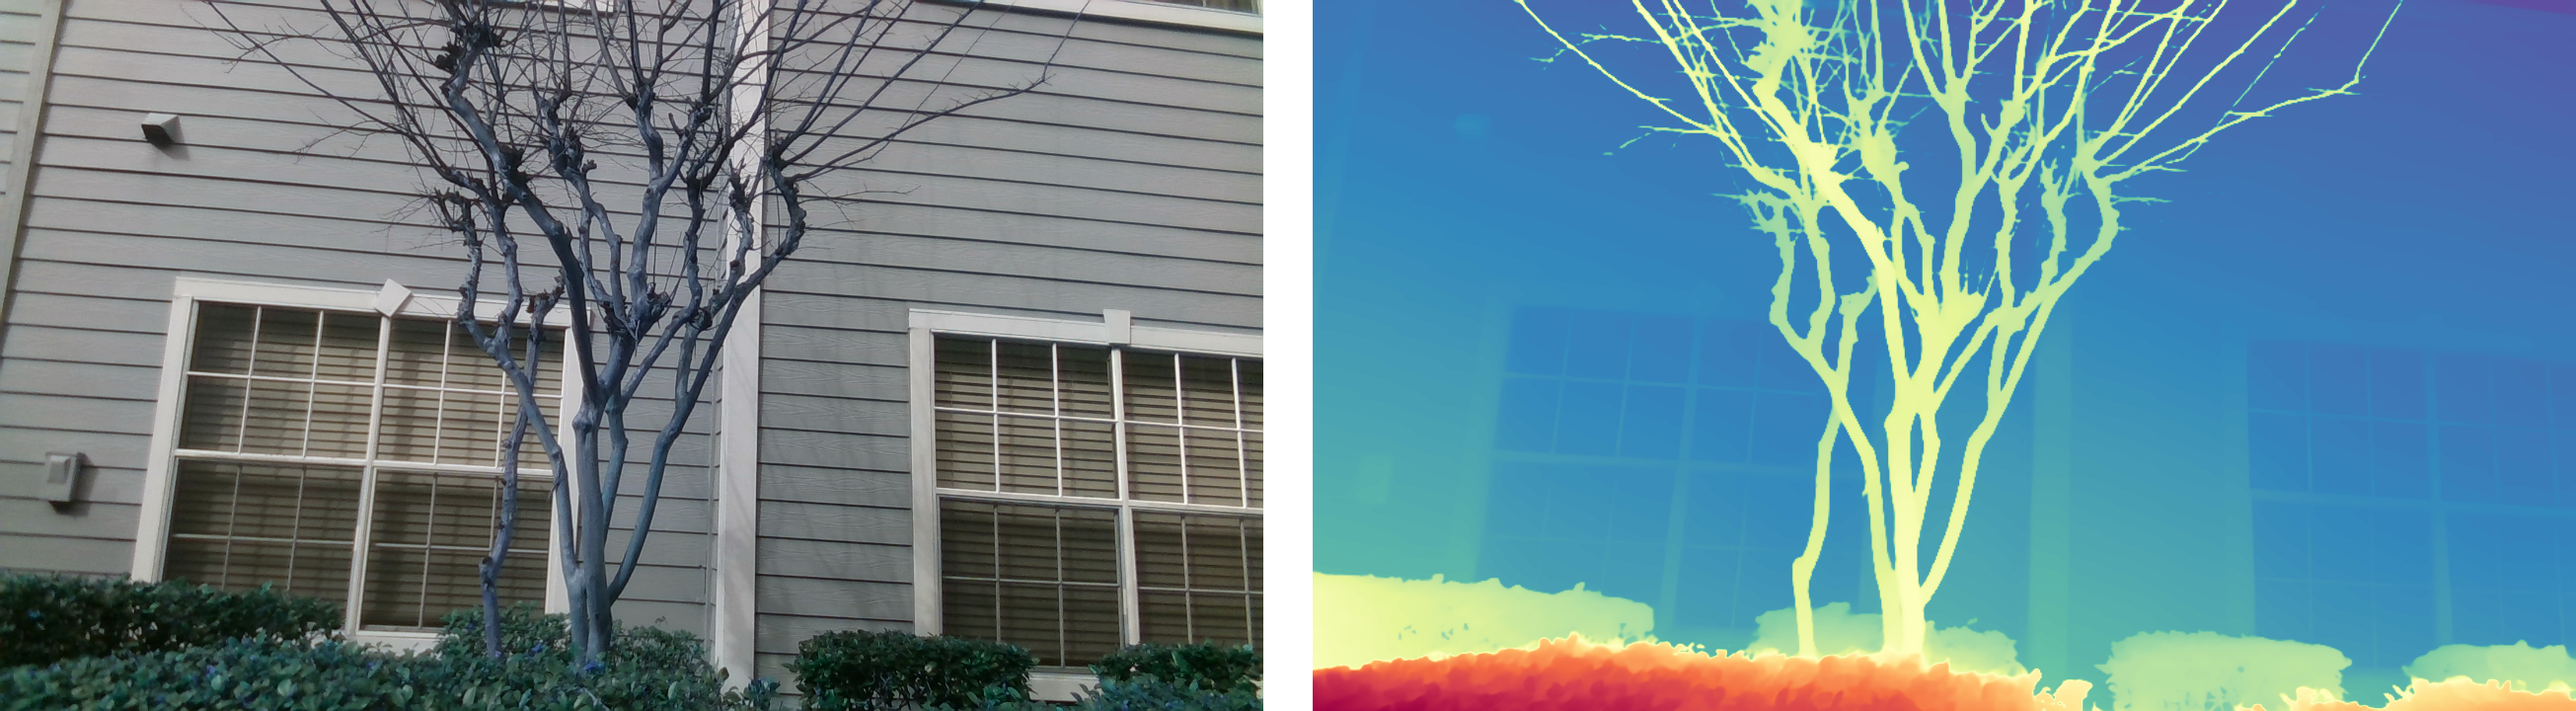
\includegraphics[width=\linewidth]{figures/depthanything_large7.png}
        \caption{Outdoor scene}
        \label{fig:da_outdoor}
    \end{subfigure}

    \caption{Depth Anything V2 results on indoor and outdoor scenes. Each panel shows the RGB input and predicted depth map.}
    \label{fig:depthanything}
\end{figure}

\FloatBarrier

\subsection{Stereo Model Evaluation}

RAFT-Stereo and HITNet both performed poorly on the tested scenes. Figure~\ref{fig:raft} shows representative RAFT-Stereo results. The outputs did not produce reliable or visually meaningful depth maps for either the indoor or outdoor scene. This poor result was not unexpected after closer inspection of the input domain. The current HypRID setup uses the RealSense D415 IR stereo pair, while these stereo models are designed around RGB stereo pairs. This mismatch between training data and testing data likely caused the models to fail on the current system input.

This result suggests that existing stereo models are not directly compatible with the present HypRID setup. A possible future solution is to build a custom RGB stereo camera system with two RGB cameras. Such a system would provide better control over the camera baseline and camera specifications, while also producing input data that better matches the expected domain of common stereo depth-estimation models.

\begin{figure}[H]
    \centering
    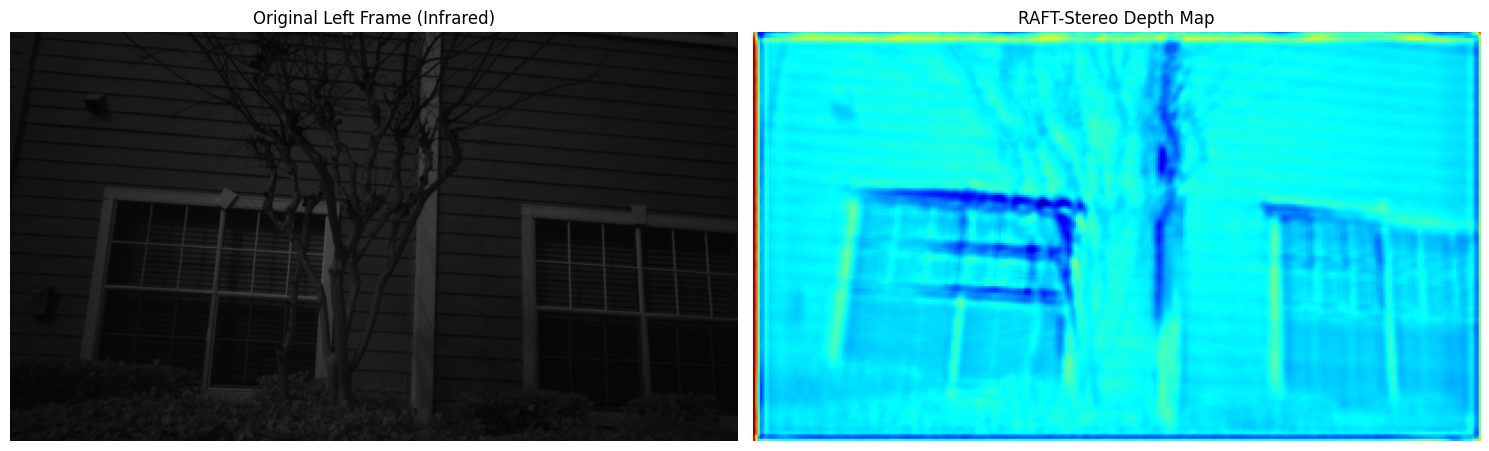
\includegraphics[width=0.95\columnwidth]{figures/RAFT.png}
    \caption{Representative RAFT-Stereo result on the outdoor tree scene. The side-by-side comparison shows the input scene and the predicted output. The poor result suggests that RGB-trained stereo models do not directly fit the current D415 IR stereo setup.}
    \label{fig:raft}
\end{figure}

\subsection{RadarHD Evaluation}

The RadarHD evaluation produced incomplete results after adapting ColoRadar data to the model input format. Figure~\ref{fig:radarhd} compares the expected output structure with the output obtained from the adapted ColoRadar pipeline. Although the model executed successfully, the result was incomplete and did not match the expected quality of the original RadarHD output.

This result suggests that radar depth-map models can be sensitive to dataset format, radar configuration, preprocessing details, and training distribution. Since the RadarHD model was not trained on ColoRadar, the poor output may be explained by both data-format mismatch and limited cross-dataset generalization. This outcome is still useful for HypRID because it indicates that future radar models should be designed together with the dataset format and sensor configuration, rather than assuming that existing radar models will transfer directly.

\begin{figure}[H]
    \centering
    \begin{subfigure}{0.48\columnwidth}
        \centering
        
\includegraphics[width=\linewidth]{figures/120_0_60_label.png}
        \caption{Expected output}
        \label{fig:radarhd_expected}
    \end{subfigure}
    \hfill
    \begin{subfigure}{0.48\columnwidth}
        \centering
        
\includegraphics[width=\linewidth]{figures/120_0_60_pred.png}
        \caption{Our output}
        \label{fig:radarhd_ours}
    \end{subfigure}
    \caption{RadarHD evaluation comparison. The expected output shows the type of complete radar depth representation targeted by RadarHD, while our output on adapted ColoRadar data is incomplete.}
    \label{fig:radarhd}
\end{figure}

\section{Discussion}

The final-stage progress changed the direction of HypRID from immediate dataset collection toward model-guided dataset planning. This shift is important because the value of the dataset depends on the task it is designed to support. Rather than collecting data first and deciding on a model later, the current work reviewed and evaluated existing RGB depth estimation, stereo depth, radar depth-map, and radar-camera fusion methods to identify a more focused future model objective.

The qualitative RGB depth estimation results suggest that Depth Anything V2 is currently the most promising depth-estimation direction among the tested models. Although its outputs are relative depth maps rather than direct metric depth measurements, they preserve object outlines, relative scene structure, thin details, and difficult visual regions better than the other tested RGB-based models. This makes Depth Anything V2 useful not necessarily as the final output model, but as a possible source of visual guidance for future multimodal fusion.

The stereo model results suggest that directly applying existing RGB-trained stereo networks to the current RealSense D415 IR image pair is not effective. Both RAFT-Stereo and HITNet produced poor outputs in the tested scenes. This does not mean stereo depth estimation is unsuitable for HypRID, but it does suggest that the sensing hardware and model assumptions need to match. If stereo information becomes important to the final system, a custom RGB stereo camera may be more appropriate than relying on the D415 IR pair.

The RadarHD evaluation also showed that radar models are sensitive to dataset and preprocessing compatibility. Even though the model ran successfully after adapting ColoRadar data, the incomplete output suggests that radar depth-map models may not generalize well without matching the radar configuration, input representation, and preprocessing pipeline used during training. This finding is directly relevant to HypRID because it reinforces the need to design the dataset format and future model architecture together.

The MetaMoran review provides the clearest direction for future HypRID model design. Its use of RGB segmentation and depth estimation to guide radar depth imaging is closely aligned with the proposed HypRID direction. However, MetaMoran uses 2D radar, which limits elevation information. HypRID can potentially extend this fusion idea by incorporating both 2D and 3D radar point clouds. The current proposed direction is therefore to use RGB images as the visual input, generate intermediate RGB-based segmentation and depth guidance, and fuse this information with radar point clouds to produce a high-resolution depth map.

The main limitations of the current project are that no final model architecture has been selected, LiDAR ground truth is not yet available, and official dataset collection has not started. The current results should therefore be interpreted as a system update and model-design study rather than as final model performance. However, the progress made after the midterm provides a clearer technical direction for the next phase of HypRID.

\section{Future Work}

Future work will focus on finalizing the model architecture and beginning model-guided dataset collection. The current model direction is to combine RGB image information with both 2D and 3D radar point clouds to generate a high-resolution depth map. RGB-based segmentation and depth estimation will be treated as intermediate guidance, while radar point clouds will provide complementary geometric information.

The sensing system also needs to be completed with LiDAR ground truth. Once the Ouster OS0-128 LiDAR is integrated, it can provide a geometric reference for evaluating future depth-map outputs. Dataset collection should then be designed around the final model goal, including scenes and objects that test the strengths and weaknesses identified in this report. These include reflective surfaces, transparent objects, thin structures, occlusion cases, and scenes where optical depth sensing is unreliable.

A later phase of the project can compare the contributions of the 76--81 GHz radar and the 300--330 GHz radar. The lower-frequency radar may provide more robust sensing, while the higher-frequency radar may provide finer spatial detail. Combining these modalities with RGB image guidance could allow HypRID to support high-resolution depth-map generation and future downstream tasks in 3D scene understanding.

\section*{Acknowledgements}

The authors would like to thank Prof. Ashutosh Sabharwal for advising this capstone project. The authors also thank Sean Farrell and Yiying Liu for their mentorship and guidance throughout the project.

\section*{CRediT Author Statement}

Steven Chen: Conceptualization, literature review, RGB depth-estimation model testing, TI board mounting, figure preparation, methodology, writing--original draft.

Yung-Hsin Tsai: RadarHD evaluation, system testing, investigation, writing--review and editing.

\bibliographystyle{IEEEtran}
\bibliography{references}

\end{document}